\documentclass[11pt,a4paper]{article}
\usepackage[margin=1in]{geometry}
\usepackage{amsmath,amssymb}
\usepackage{graphicx}
\usepackage{booktabs}
\usepackage{caption}
\usepackage{enumitem}
\usepackage{listings}
\usepackage{hyperref}
\usepackage{microtype}
\graphicspath{{figures/}}
\hypersetup{hidelinks}
\lstset{basicstyle=\small\ttfamily,breaklines=true,columns=fullflexible}

\title{Wobble-Suppressed Calibration of Mean-Pole Polar Motion}
\author{Craig Stone}
\date{November 2026}

\begin{document}
\maketitle

\begin{abstract}
The Earth Orientation Parameter record carries Chandler and annual wobble and a secular mean-pole drift. Three EOP products (IERS finals, JPL EOP2, C04) are smoothed with a centered moving average of half-window two years (a four-year boxcar width) and rates are estimated by ordinary least squares with block-bootstrap intervals. The early era runs at 3.6--5.0 mas/yr, the middle calendar window 2010--2020 at 4.6 mas/yr, and the burst centered width reads 5.9 mas/yr (18.1 cm/yr) but is unstable: the half-width sweep from 1.0 to 3.0 years gives 8.1 down to 2.7 mas/yr, a local harmonic fit over the last 4.1 years gives 8.7 mas/yr, and longer baselines give raw OLS 4.5 (2000--end), 5.2 (2010--end) and calendar-year means 3.7--4.7 (2020--2026). The data support roughly 4--5 mas/yr since about 2000, not a distinct 18 cm/yr episode. The raw 20.0 mas/yr is a Chandler-leakage artifact: the 4.12-year window is near a half-integer Chandler cycle, while whole multiples give 20.3 (2.37 yr), 5.7 (3.55 yr) and 4.9 (4.74 yr). A baseline residual of raw OLS 2010--end minus the known climate+GIA budget leaves 0.8 mas/yr (CI 0.35--4.1), consistent with zero to about 1 mas/yr; the benchmark overlaps 2010--2020 and is not an independent test. Net displacement is 5.94, 7.18 and 7.59 m; the recent yearly-mean addition is 0.74 m and approximate. The dated snapshot, checksums, script and public repository reproduce every number.
\end{abstract}

\section{Purpose and scope}

Polar motion is measured as the displacement of the Earth's rotation pole over the surface, reported as $x_{\text{pole}}$ and $y_{\text{pole}}$ in arcseconds. Two components sit in that record: the Chandler wobble (period near 432.9 days) and the annual wobble (365.2425 days), both returning on themselves within metres, and a secular drift that accumulates over decades. A rate computed from a short window without suppressing the wobble inflates the secular drift: the raw example is about 3.4 times the smoothed rate and sequential subtraction about 1.8 times. This paper calibrates the secular component, states the failure modes and the edge limitations explicitly, and provides the snapshot, script and repository needed to reproduce every number.

The scope is the observed record and its calibration. No mechanism, coupling, or causal claim is made or tested here. Surface mass redistribution provides the physical context for polar motion \cite{adhikari}. Section 7 subtracts the published climate+GIA budget as a benchmark, but that subtraction is not a mechanism test and does not establish causation.

\section{Data sources}

The DRIFT dashboard serves Earth Orientation Parameter series from three products at \url{http://mac-studio:3111/api/eop?dataset=<id>}. Dataset identifiers are \texttt{finals} (IERS finals.all IAU1980, the operational default), \texttt{jpl} (JPL EOP2), and \texttt{c04} (EOP 20u24 C04 IAU2000A). The response fields used are \texttt{t}, \texttt{xp} and \texttt{yp}; unknown or omitted dataset values fall back to \texttt{finals}. Source freshness is reported by \texttt{/api/eop-source-notice}; on 24 November 2026 the default IERS product was active with latest sample 2026-11-22 and zero lag days.

{\sloppy
The upstream products are public: the IERS Earth Orientation Center at \url{https://datacenter.iers.org} and JPL EOP2 at \url{https://eop2-external.jpl.nasa.gov/eop2/latest_eop2.long}. The three products draw on the same VLBI, GPS and SLR observational base; they are different reductions of one measurement system, so agreement across them is consistency rather than independent corroboration. Before 1973 the JPL and C04 series include optical astrometry with errors of tens of milliarcseconds, comparable to the metre-scale differences in net displacement reported below.
\par}

\begin{table}[ht]
\centering
\caption{Series inventory pulled from the live DRIFT endpoint on 24 November 2026.}
\label{tab:inventory}
\begin{tabular}{lrrll}
\toprule
Dataset & Records & Start & End & Latest sample \\
\midrule
IERS finals & 19{,}683 & 1973-01-02 & 2026-11-22 & 2026-11-22 \\
JPL EOP2 & 23{,}683 & 1962-01-20 & 2026-11-22 & 2026-11-22 \\
C04/IAU2000A & 23{,}702 & 1962-01-01 & 2026-11-22 & 2026-11-22 \\
\bottomrule
\end{tabular}
\end{table}

\section{Units and surface conversion}

Polar motion coordinates are reported in arcseconds. One milliarcsecond (mas) of polar motion corresponds to a surface displacement of approximately 3.09 cm, obtained from the Earth's mean radius $R = 6371$ km:
\begin{equation}
c_{\text{cm per mas}} = R_{\text{km}} \times 10^{5} \times \frac{10^{-3}}{206\,264.80625} \approx 3.09 \text{ cm}.
\end{equation}
A rate $r$ in mas/yr therefore maps to surface drift as $r \times 3.09$ cm/yr. Rates in this paper are reported in mas/yr and cm/yr, with in/yr and ft/yr where useful; one foot is 30.48 cm.

\section{Wobble suppression methodology}

\subsection{Period units}

The wobble periods are quoted in days: annual 365.2425, semiannual 182.6211, Chandler 432.9. The time axis of the record is in years, so a sinusoid frequency must use periods in years: 1.0, 0.5 and 432.9/365.2425 $\approx$ 1.185. A one-basis least-squares fit of constant, linear trend and those sinusoids over the whole record returns 3.2 mas/yr (9.9 cm/yr), consistent with the early-era rate. This is a whole-record secular estimate, not a burst-window value.

\subsection{Residual wobble and the raw window}

Sequential sinusoid subtraction --- fit the linear trend first, then fit harmonics to the residual and subtract them --- leaves residual Chandler and annual leakage because amplitude and phase drift across the record. A daily-window slope over the recent window then reads 10.7 mas/yr (33.1 cm/yr), roughly twofold the smoothed secular rate. A raw daily-window slope reads 20.0 mas/yr (61.6 cm/yr) in this one window, but raw trailing slopes swing from 1.5 to 22.8 mas/yr and read 5.0 at the series end; 20.0 is one example of that scatter, not the raw secular rate. Both raw and sequential values are wobble inflation.

\begin{table}[ht]
\centering
\caption{Method contrast on the IERS finals October 2022--November 2026 window. The whole-record co-fit is context; the raw and sequential rows show wobble inflation; the smoothed row is the secular estimate, with its edge variant.}
\label{tab:contrast}
\small
\resizebox{\textwidth}{!}{%
\begin{tabular}{lrrl}
\toprule
Method & Rate (mas/yr) & Rate (cm/yr) & Status \\
\midrule
Raw daily-window slope & 20.0 & 61.6 & One example of raw scatter (range 1.5--22.8) \\
Whole-record one-basis co-fit & 3.2 & 9.9 & Whole-record rate, periods in years \\
Sequential sinusoid subtraction & 10.7 & 33.1 & Residual wobble leakage \\
Centered smoothing (full window) & 5.9 & 18.1 & Secular estimate, CI 3.6--8.6 \\
Centered smoothing (interior, excl last 2 yr) & 3.8 & 11.7 & Edge variant, ~2.1-yr window; noisy \\
\bottomrule
\end{tabular}}
\end{table}

\subsection{Centered smoothing and its edge limits}

The suppressor is a centered moving average over half-window two years either side of each sample:
\begin{equation}
S(t_i) = \frac{1}{N_i} \sum_{j:\,|t_j - t_i| \le 2\text{ yr}} x_j .
\end{equation}
The full width is four years; the Chandler period is 432.9 days, about 1.186 years, and a four-year width spans multiple Chandler cycles, averaging out the annual and semiannual components. Two limits are stated explicitly. First, samples within two years of either end of the series use truncated windows: annual leakage appears there because the width is no longer an integer number of years, and Chandler suppression is imperfect even in the interior. Second, the burst window ends at the series end, so its last two years carry truncated windows. Edge truncation makes the burst estimate unstable rather than inflating it uniformly: the full-window 5.9 mas/yr and interior-only 3.8 mas/yr are not a stable ordering across widths, and the four-year window is too short to fix the rate.

\subsection{Burst sensitivity and Chandler-multiple windows}

The burst rate is one point on a steep curve, not a robust estimate. A half-width sweep for IERS finals gives:

\begin{table}[ht]
\centering
\caption*{Burst rate vs centered smoothing half-width, IERS finals.}
\begin{tabular}{rrr}
\toprule
Half-width (yr) & Full window (mas/yr) & Interior-only (mas/yr) \\
\midrule
1.0 & 8.1 & 11.2 \\
1.19 (one Chandler cycle) & 9.5 & 15.2 \\
2.0 (paper) & 5.9 & 3.8 \\
2.37 (two Chandler cycles) & 5.0 & n/a \\
3.0 & 2.7 & n/a \\
\bottomrule
\end{tabular}
\end{table}

A local harmonic fit over the last $N$ years is also unstable: 8.7 mas/yr for 4.1 years, 8.2 for 5, 6.1 for 6, 4.2 for 8 and 3.7 for 10. The four-year burst window cannot separate drift from Chandler phase. Longer baselines show no distinct recent episode:

\begin{table}[ht]
\centering
\caption*{Raw OLS rates by window length, baseline and harmonic fit, IERS finals.}
\begin{tabular}{llr}
\toprule
Category & Window or baseline & Rate (mas/yr) \\
\midrule
Raw OLS & 2.37 yr ending at series end & 20.3 \\
Raw OLS & 3.55 yr ending at series end & 5.7 \\
Raw OLS & 4.12 yr ending at series end & 19.9 \\
Raw OLS & 4.74 yr ending at series end & 4.9 \\
Raw OLS & 2000--end & 4.5 \\
Raw OLS & 2010--end & 5.2 \\
Raw OLS & 2015--end & 5.1 \\
Calendar-year means & 2018--2026 & 4.0 \\
Calendar-year means & 2020--2026 & 3.7 \\
Calendar-year means & 2022--2026 & 4.7 \\
Harmonic fit & last 4.1 yr & 8.7 \\
Harmonic fit & last 5 yr & 8.2 \\
Harmonic fit & last 6 yr & 6.1 \\
Harmonic fit & last 8 yr & 4.2 \\
Harmonic fit & last 10 yr & 3.7 \\
\bottomrule
\end{tabular}
\end{table}

\begin{figure}[ht]
\centering
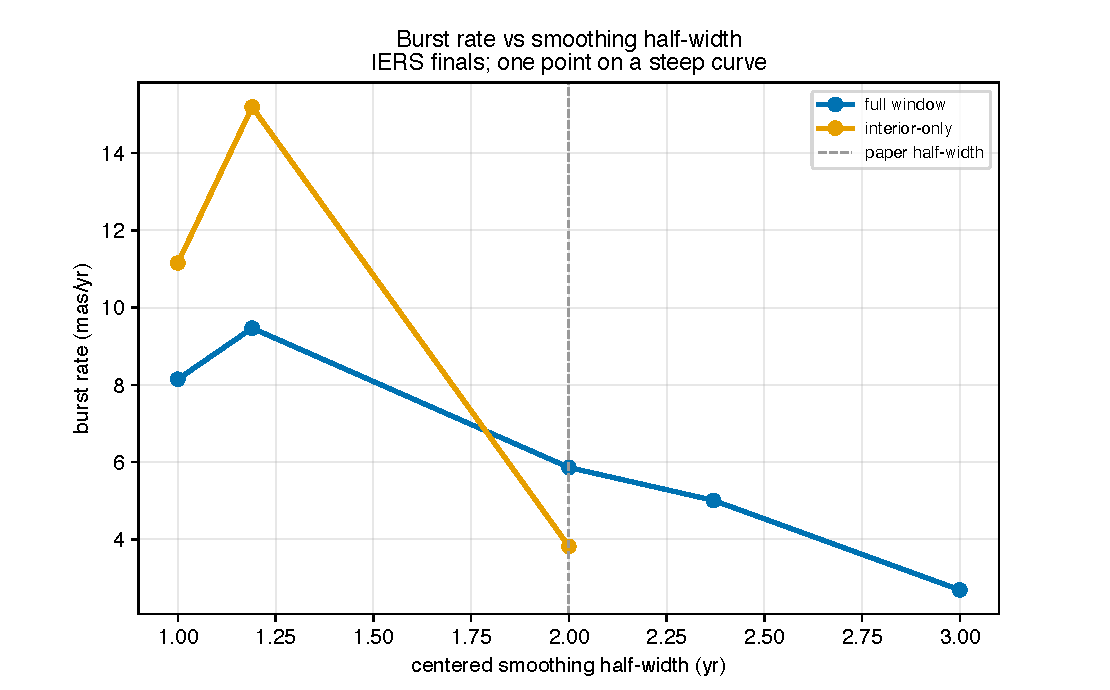
\includegraphics[width=0.9\textwidth]{figures/fig8_halfwidth_sweep.pdf}
\caption*{Burst rate vs smoothing half-width, IERS finals. The 5.9 mas/yr paper value is one point on a steep curve between about 9 and 3 mas/yr.}
\end{figure}

\begin{figure}[ht]
\centering
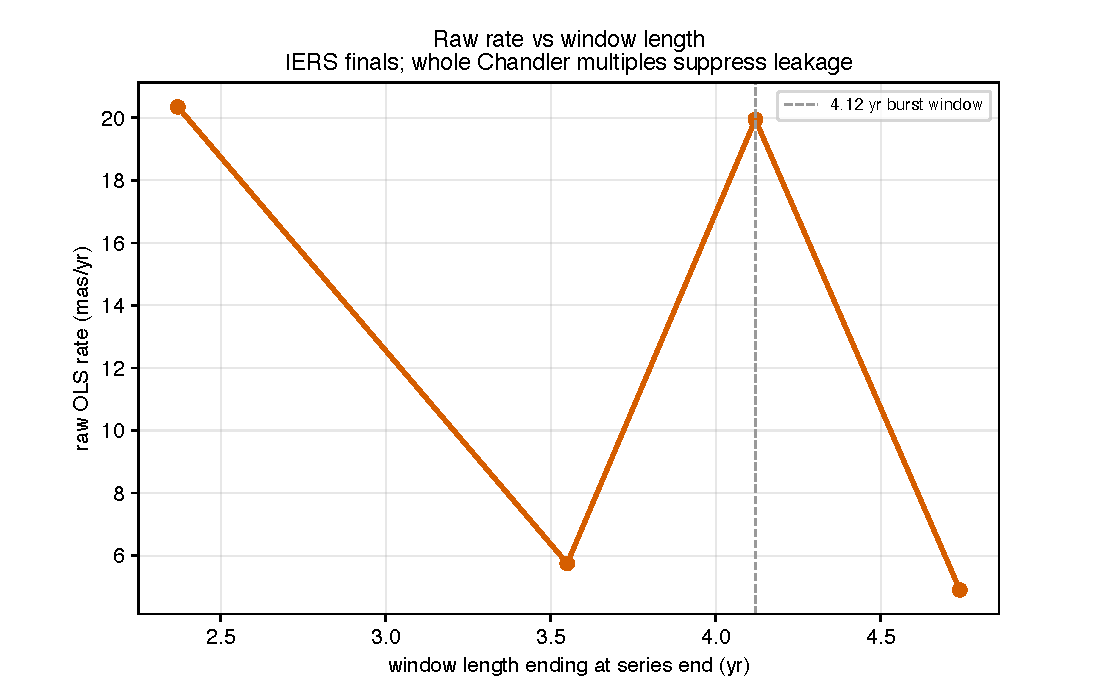
\includegraphics[width=0.9\textwidth]{figures/fig9_chandler_windows.pdf}
\caption*{Raw OLS rate vs window length ending at the series end, IERS finals. Whole Chandler multiples give 5--6 mas/yr; the 4.12-year burst window sits near a half-integer cycle and reads 19.9 mas/yr.}
\end{figure}

The raw 20.0 mas/yr is therefore a Chandler-leakage artifact, not a secular burst: a window of 4.12 years is near a half-integer number of Chandler cycles, the worst case for leakage, while whole multiples suppress it. Longer baselines give roughly 4--5 mas/yr since about 2000--2010, consistent with the middle-era 4.6 mas/yr; the data do not support 18 cm/yr as a distinct recent episode. A half-width sweep or Chandler-multiple windows are a stronger robustness check than the bootstrap, because the bootstrap cannot capture the sensitivity to window choice.

\section{Epoch definition and rate estimation}

The early window is $(t_0, t_0+33)$ years and is dataset-specific: 1973--2006 for IERS finals and 1962--1995 for JPL and C04. The middle window is the common calendar interval 2010--2020 for all three products, so the rates compare like intervals. The burst window is $(t_e-4.12, t_e)$, the October 2022 to November 2026 interval. The boundaries are exploratory and arbitrary; the burst window was chosen after observing the recent episode, not pre-registered.

Within each window a linear model $x(t) = a + bt$ is fitted by ordinary least squares to the smoothed series. The slope $b$ is converted to mas/yr by multiplying by $10^3$. The combined drift magnitude is
\begin{equation}
r = \sqrt{(b_x \times 10^3)^2 + (b_y \times 10^3)^2}.
\end{equation}
Uncertainty is estimated by a block bootstrap: 2-year blocks (~730 samples) of the smoothed series are resampled with replacement, 3000 replicates are fitted with a per-call seed, and the 2.5th and 97.5th percentiles are reported. The smoothed series is autocorrelated, and the bootstrap does not capture the systematic edge bias, so these intervals are approximate and do not carry the assumptions of ordinary least-squares standard errors.

The drift longitude uses the east-positive convention:
\begin{equation}
\lambda = \operatorname{atan2}(-b_y, b_x),
\end{equation}
where $\lambda$ is measured eastward from Greenwich and negative values denote west. The reported azimuths are signed longitudes: $-73.6$ degrees means 73.6 degrees west, not a "westward convention" that hides the sign.

\section{Results}

\begin{table}[ht]
\centering
\caption{Secular mean-pole drift rates per epoch with block-bootstrap intervals, from the centered smoothing. Azimuth is signed longitude, east-positive; negative values are west. The burst row is one centered half-width; the sensitivity sweep shows the estimate is unstable.}
\label{tab:rates}
\small
\resizebox{\textwidth}{!}{%
\begin{tabular}{llrrrrrr}
\toprule
Dataset & Epoch & $b_x$ & $b_y$ & Rate (mas/yr) & Bootstrap CI & cm/yr & Azimuth \\
\midrule
IERS finals & Early (1973--2006) & 1.0 & 3.4 & 3.6 & 3.1--4.0 & 11.0 & $-73.6$ \\
IERS finals & Middle (2010--2020) & 4.1 & 2.1 & 4.6 & 4.6--6.2 & 14.3 & $-26.7$ \\
IERS finals & Burst (Oct 2022--Nov 2026) & 3.8 & 4.5 & 5.9 & 3.6--8.6 & 18.1 & $-50.1$ \\
JPL EOP2 & Early (1962--1995) & 2.3 & 4.1 & 4.7 & 4.5--5.2 & 14.5 & $-61.1$ \\
JPL EOP2 & Middle (2010--2020) & 4.1 & 2.1 & 4.6 & 4.6--6.1 & 14.3 & $-26.8$ \\
JPL EOP2 & Burst (Oct 2022--Nov 2026) & 3.8 & 4.5 & 5.9 & 3.7--8.6 & 18.1 & $-50.2$ \\
C04/IAU2000A & Early (1962--1995) & 2.0 & 4.6 & 5.0 & 4.8--5.4 & 15.6 & $-66.1$ \\
C04/IAU2000A & Middle (2010--2020) & 4.1 & 2.1 & 4.6 & 4.6--6.1 & 14.3 & $-26.7$ \\
C04/IAU2000A & Burst (Oct 2022--Nov 2026) & 3.8 & 4.5 & 5.9 & 3.7--8.6 & 18.1 & $-50.2$ \\
\bottomrule
\end{tabular}}
\end{table}

\begin{table}[ht]
\centering
\caption{Net mean-pole displacement from the smoothed yearly-mean positions, measured from the first yearly mean to the last, with the recent-window addition. The 2022--2026 increment uses yearly means that include the truncated end, so it likely carries the same upward edge bias and is approximate.}
\label{tab:net}
\begin{tabular}{llrrr}
\toprule
Dataset & Span & Displacement (m) & Displacement (ft) & 2022--2026 adds (m) \\
\midrule
IERS finals & 1973--2026 & 5.94 & 19.5 & 0.74 \\
JPL EOP2 & 1962--2026 & 7.18 & 23.6 & 0.74 \\
C04/IAU2000A & 1962--2026 & 7.59 & 24.9 & 0.74 \\
\bottomrule
\end{tabular}
\end{table}

\begin{figure}[ht]
\centering
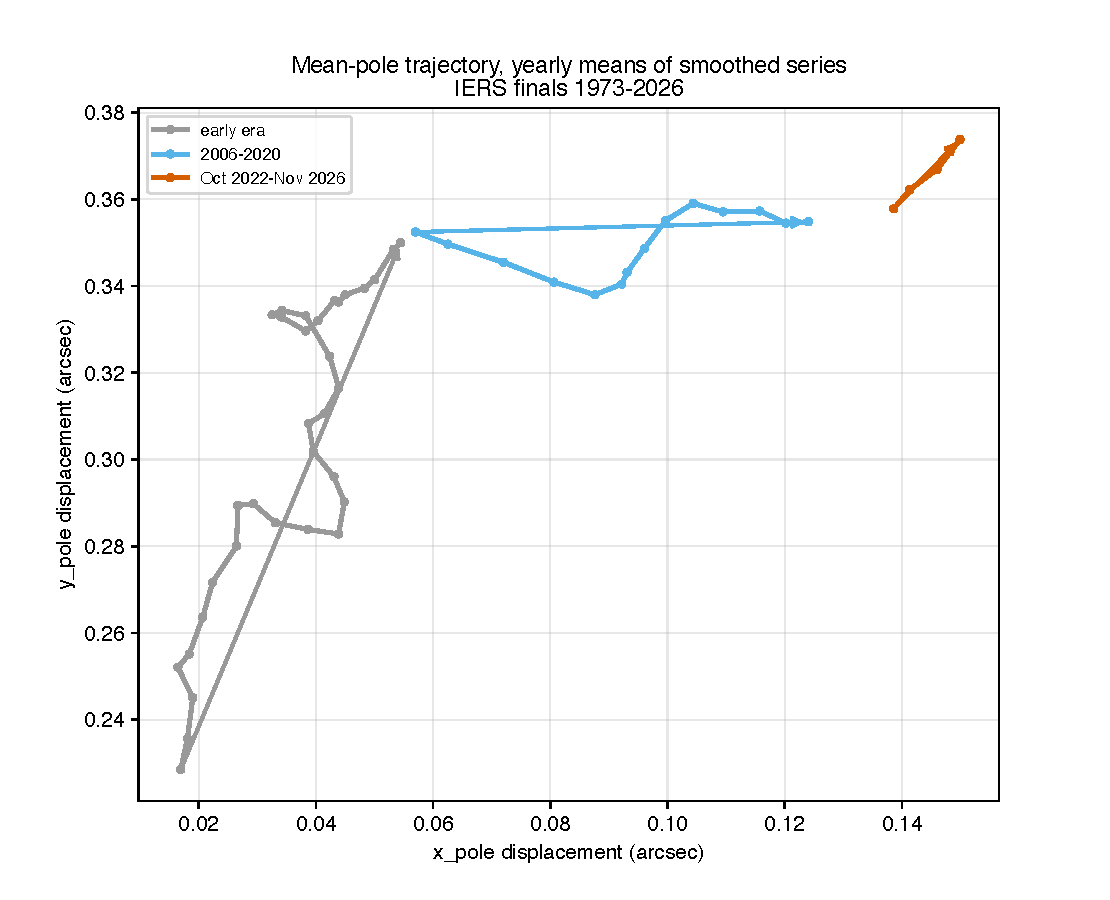
\includegraphics[width=0.9\textwidth]{figures/fig1_trajectory.pdf}
\caption{Mean-pole trajectory plotted as displacement from the 1973 first yearly mean of the smoothed IERS finals series, 1973--2026. Epoch segments are coloured and arrows mark net displacement within each epoch; the early drift longitude is about $-73.6$ degrees (west).}
\label{fig:trajectory}
\end{figure}

\begin{figure}[ht]
\centering
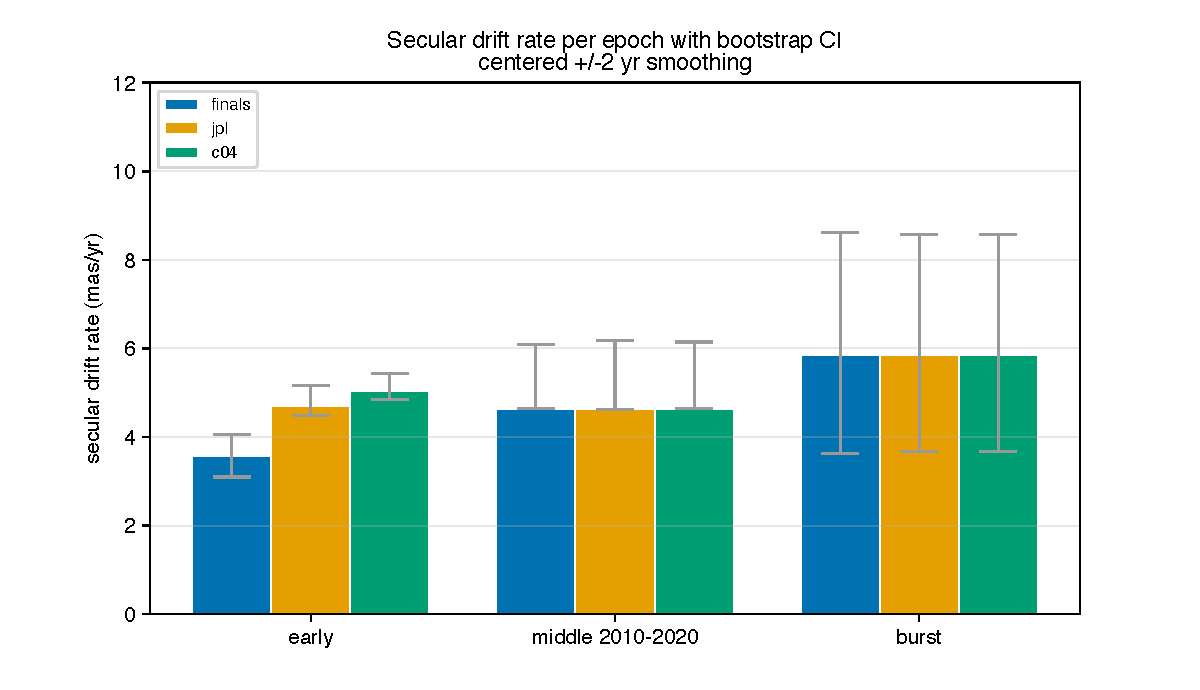
\includegraphics[width=0.9\textwidth]{figures/fig2_epoch_rates.pdf}
\caption{Secular drift rate per epoch with block-bootstrap intervals for IERS finals, JPL EOP2 and C04. The burst window reads 5.9 mas/yr (18.1 cm/yr) at half-width two years in all three products, with intervals 3.6--8.6, 3.7--8.6 and 3.7--8.6; the sensitivity sweep spans 8.1--2.7 mas/yr, so this is an unstable centered-width value rather than a robust rate. The early-era spread reflects the different record spans (1973 versus 1962 starts).}
\label{fig:rates}
\end{figure}

\begin{figure}[ht]
\centering
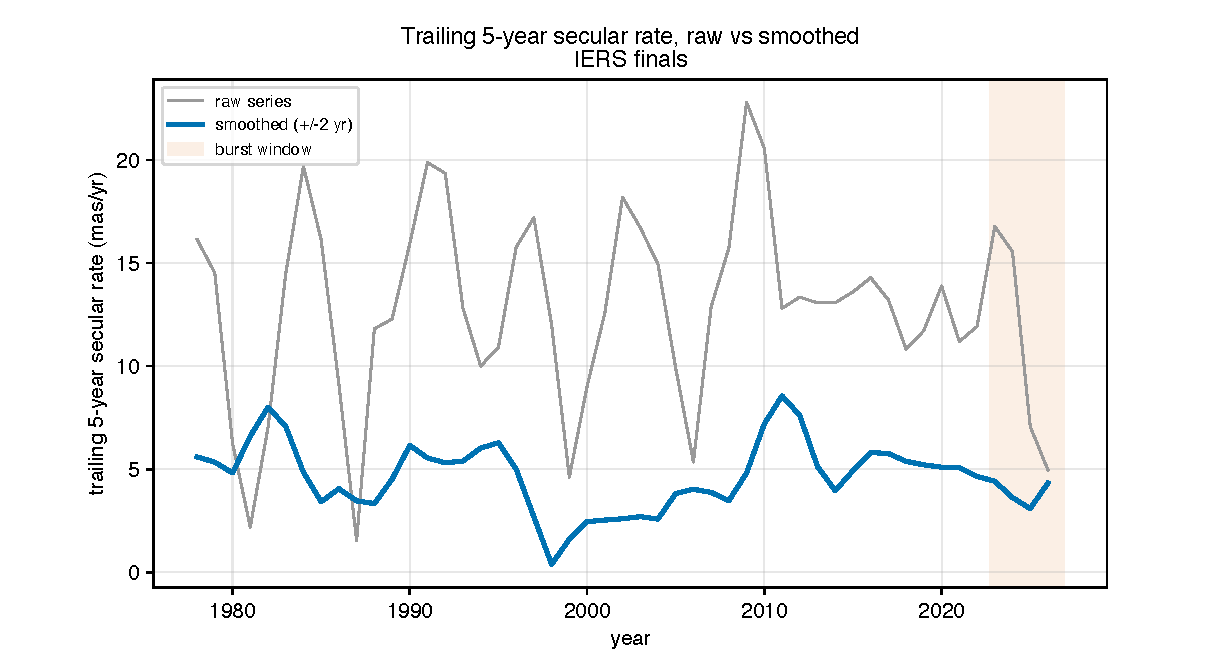
\includegraphics[width=0.9\textwidth]{figures/fig3_rolling_rate.pdf}
\caption{Trailing five-year secular rate for the raw series versus the centered smoothed series, IERS finals. Raw short-window slopes swing from 1.5 to 22.8 mas/yr (maximum at 2009) and read 5.0 at the series end; the smoothed series peaks near 8.6 mas/yr at 2011 and its trailing values in 2022--2026 fall to 3.1--4.7 mas/yr, below the full-window burst estimate of 5.9. The point estimates 3.6, 4.6 and 5.9 are monotonic, but their intervals overlap and this rolling series does not support a trend; the burst figure is sensitive to window choice.}
\label{fig:rolling}
\end{figure}

\begin{figure}[ht]
\centering
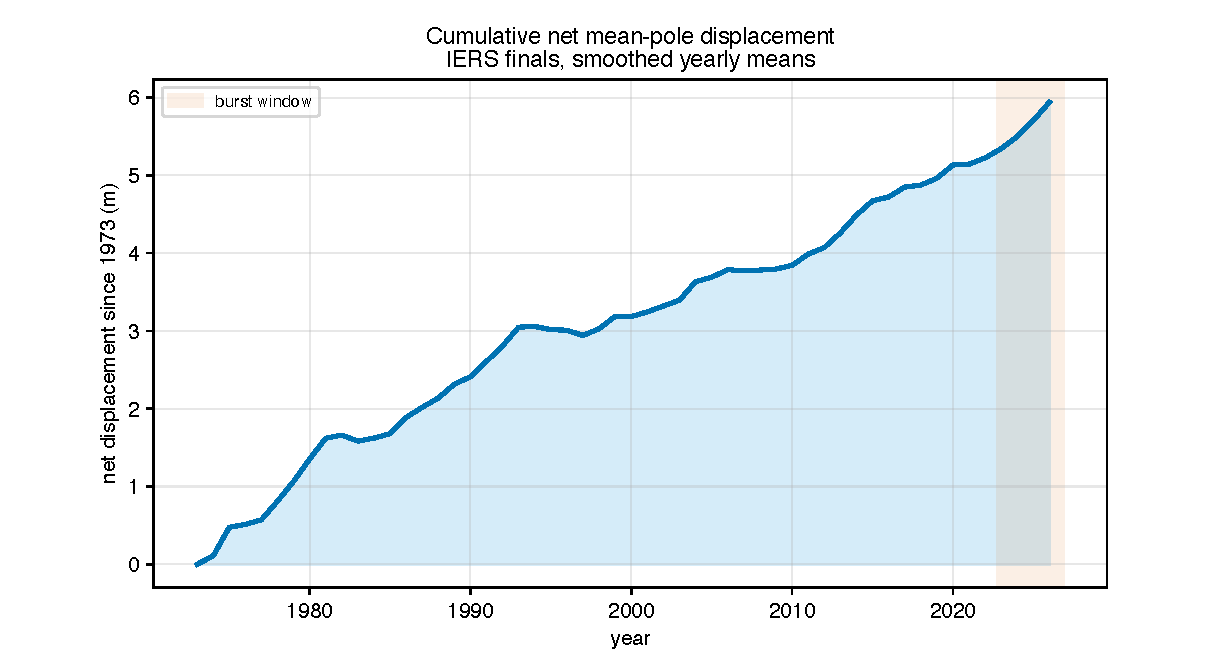
\includegraphics[width=0.9\textwidth]{figures/fig4_cumulative.pdf}
\caption{Cumulative net mean-pole displacement from smoothed yearly means, IERS finals 1973--2026. The total is 5.94 m (19.5 ft); the 2022--2026 yearly-mean increment is 0.74 m, which includes the truncated end and is approximate.}
\label{fig:cumulative}
\end{figure}

\section{Residual after subtracting known contributions}

The observed secular vectors are compared against the known contributions reported by Adhikari and Ivins (2016) for the 2003--2015 climate-driven polar motion. Their reconstruction partitions polar motion into cryospheric (GIS, AIS, global glaciers), terrestrial water storage (TWS), and atmospheric/ocean mass (AOM) components. The full climate reconstruction is 4.56 $\pm$ 1.26 mas/yr along 27.7 $\pm$ 7.6$^{\circ}$E and explains 82.6 $\pm$ 22.8\% of the detrended observed motion; the cryosphere alone is 3.65 $\pm$ 0.38 mas/yr along 4.4 $\pm$ 11.4$^{\circ}$W. The long-term GIA trend used in that study is 0.85$^{\circ}$/Myr, which converts to 3.06 mas/yr along 75$^{\circ}$W.

\begin{table}[ht]
\centering
\caption{Known polar-motion contributions used as the subtraction benchmark, from Adhikari and Ivins (2016). Only the terms used in the subtraction are listed; the GIS, AIS and TWS partitions are not independently used here.}
\label{tab:known}
\small
\resizebox{\textwidth}{!}{%
\begin{tabular}{lrrl}
\toprule
Component & Magnitude (mas/yr) & Direction & Note \\
\midrule
Climate reconstruction (cryosphere+TWS+AOM) & $4.56\pm1.26$ & $27.7\pm7.6^{\circ}$E & Explains $82.6\pm22.8\%$ of detrended 2003--2015 motion \\
Cryosphere only (GIS+AIS+glaciers) & $3.65\pm0.38$ & $4.4\pm11.4^{\circ}$W & Explains $66.0\pm6.8\%$ of detrended motion \\
GIA long-term trend & $3.06$ & $75^{\circ}$W & $0.85^{\circ}$/Myr converted to mas/yr \\
\bottomrule
\end{tabular}}
\end{table}

Vector subtraction removes the climate reconstruction and the GIA trend from the observed vector. In the paper's frame the y axis points toward 90$^{\circ}$W, so west directions carry positive $b_y$ and east directions negative $b_y$. The baseline residual uses raw OLS over 2010 to the series end: the observed vector is about (4.9, 1.6) mas/yr and the known vector is (4.83, 0.84) mas/yr, leaving about (0.1, 0.8), or 0.77 mas/yr at $-84^{\circ}$. Early-era residuals are not reported: subtracting the 2003--2015 ice-melt budget from 1973--2006 data measures how different the early period was from the modern budget, not what remains unexplained.

The baseline overlaps the benchmark period. The climate reconstruction was derived from 2003--2015 and the baseline runs from 2010, so the subtraction is not an independent test; it measures consistency with the known budget over an overlapping interval, not unexplained motion. The climate-error-propagated bootstrap gives a residual magnitude interval of 0.35--4.08 mas/yr and about 22\% of replicates below 1 mas/yr, so the baseline residual is consistent with zero to about 1 mas/yr. The four-year burst residual is unstable, as the sensitivity sweep shows, and is not used as the headline; earlier interior-only and full-window residual values are illustrative of that instability rather than a robust claim.

\begin{table}[ht]
\centering
\caption{Baseline residual after subtracting the known climate+GIA budget from raw OLS 2010--end, with climate-error-propagated 95\% intervals. The benchmark overlaps 2010--2020, so this is not an independent test; early-era rows are omitted; the unstable four-year burst residual is not reported here.}
\label{tab:residual}
\small
\resizebox{\textwidth}{!}{%
\begin{tabular}{llrrr}
\toprule
Dataset & Baseline & Observed (mas/yr) & Residual (mas/yr, 95\% CI) & Azimuth ($^{\circ}$) \\
\midrule
IERS finals & Raw OLS 2010--2026 & 5.2 & 0.8 (0.35--4.08) & $-83.9$ \\
JPL EOP2 & Raw OLS 2010--2026 & 5.2 & 0.8 (0.30--4.14) & $-84.3$ \\
C04/IAU2000A & Raw OLS 2010--2026 & 5.2 & 0.8 (0.28--4.03) & $-83.9$ \\
\bottomrule
\end{tabular}}
\end{table}

\begin{figure}[ht]
\centering
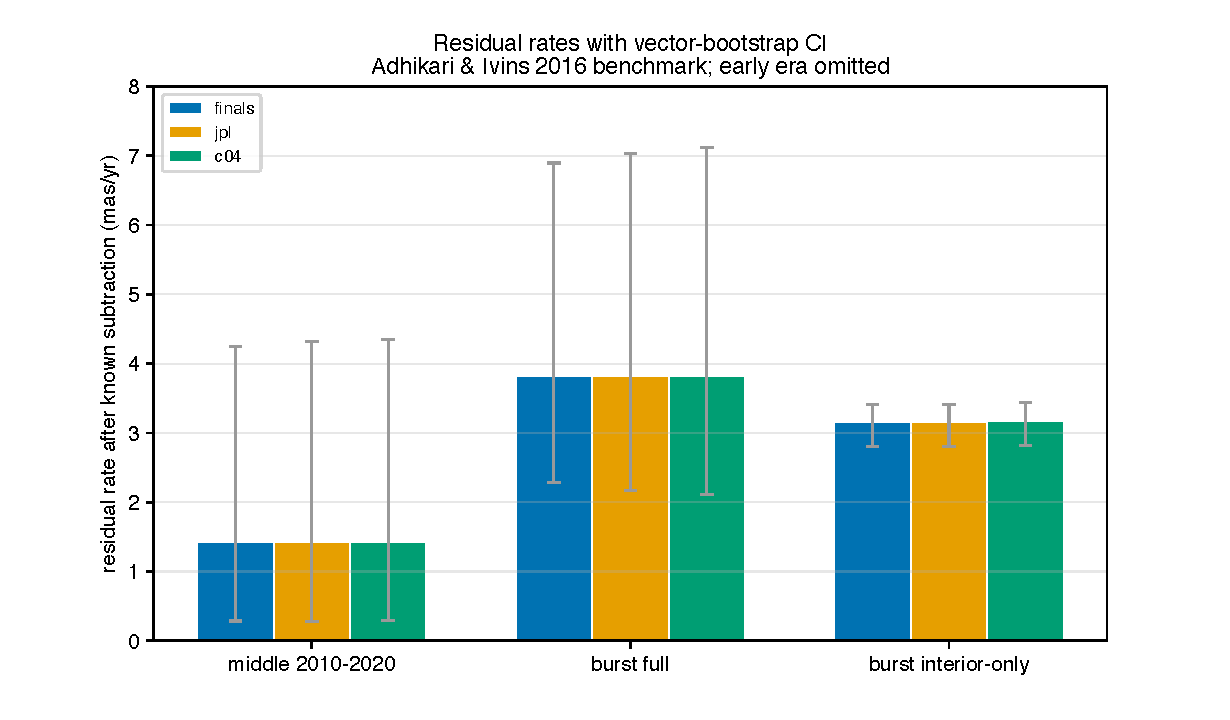
\includegraphics[width=0.9\textwidth]{figures/fig5_residual.pdf}
\caption{Baseline residual rates from raw OLS 2010--end with climate-error-propagated 95\% intervals. The residual is about 0.8 mas/yr with intervals 0.35--4.08, 0.30--4.14 and 0.28--4.03 mas/yr; about 22\% of replicates fall below 1 mas/yr, so the baseline residual is consistent with zero to about 1 mas/yr. The benchmark overlaps 2010--2020 and is not an independent test. The unstable four-year burst residual is not plotted.}
\label{fig:residual}
\end{figure}

\begin{figure}[ht]
\centering
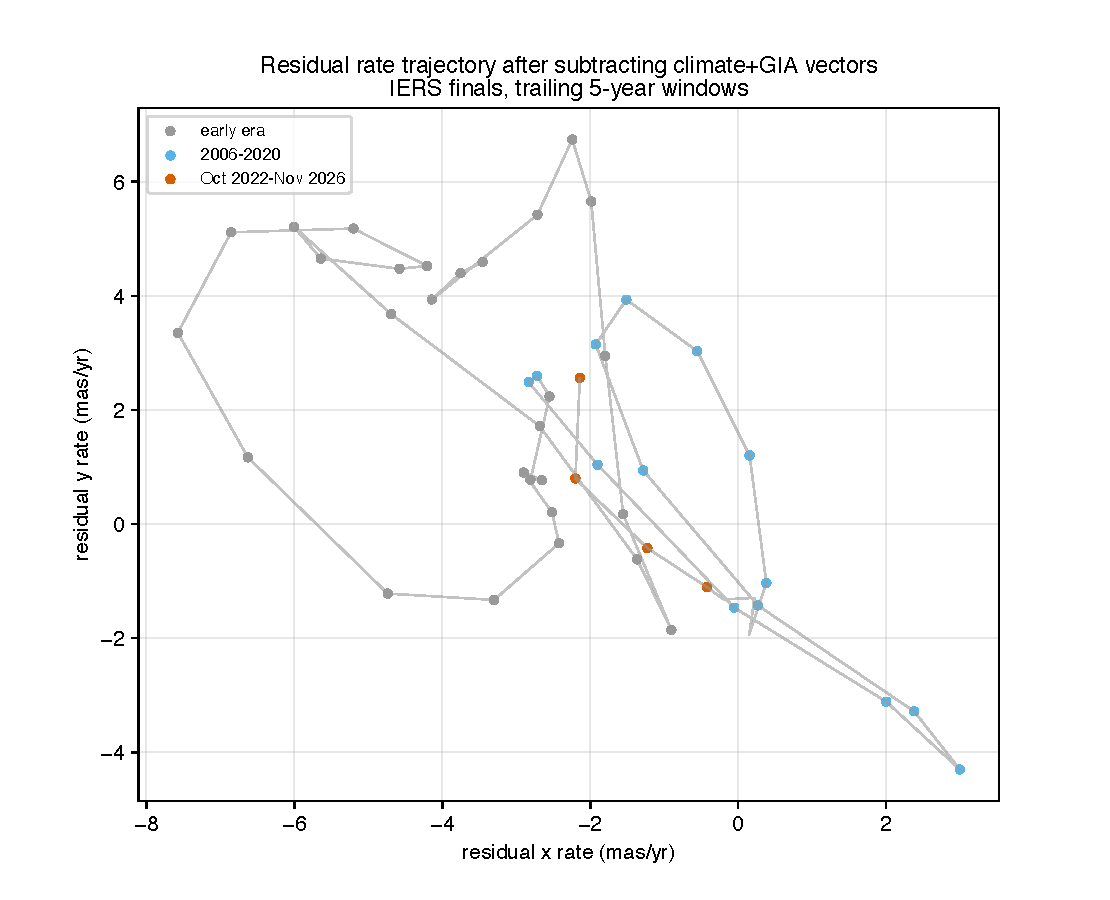
\includegraphics[width=0.9\textwidth]{figures/fig6_residual_trajectory.pdf}
\caption{Residual rate trajectory in rate space from trailing five-year window rates after subtracting the known climate+GIA vectors, IERS finals; early-era points are dropped as anachronistic. This is illustrative of the scatter, not a headline estimate: the four-year burst residual is unstable and the trajectory does not establish a resolved residual. The known climate values are measured for 2003--2015 and applied as a benchmark; the residual includes unmodelled processes.}
\label{fig:residual-trajectory}
\end{figure}

\begin{figure}[ht]
\centering
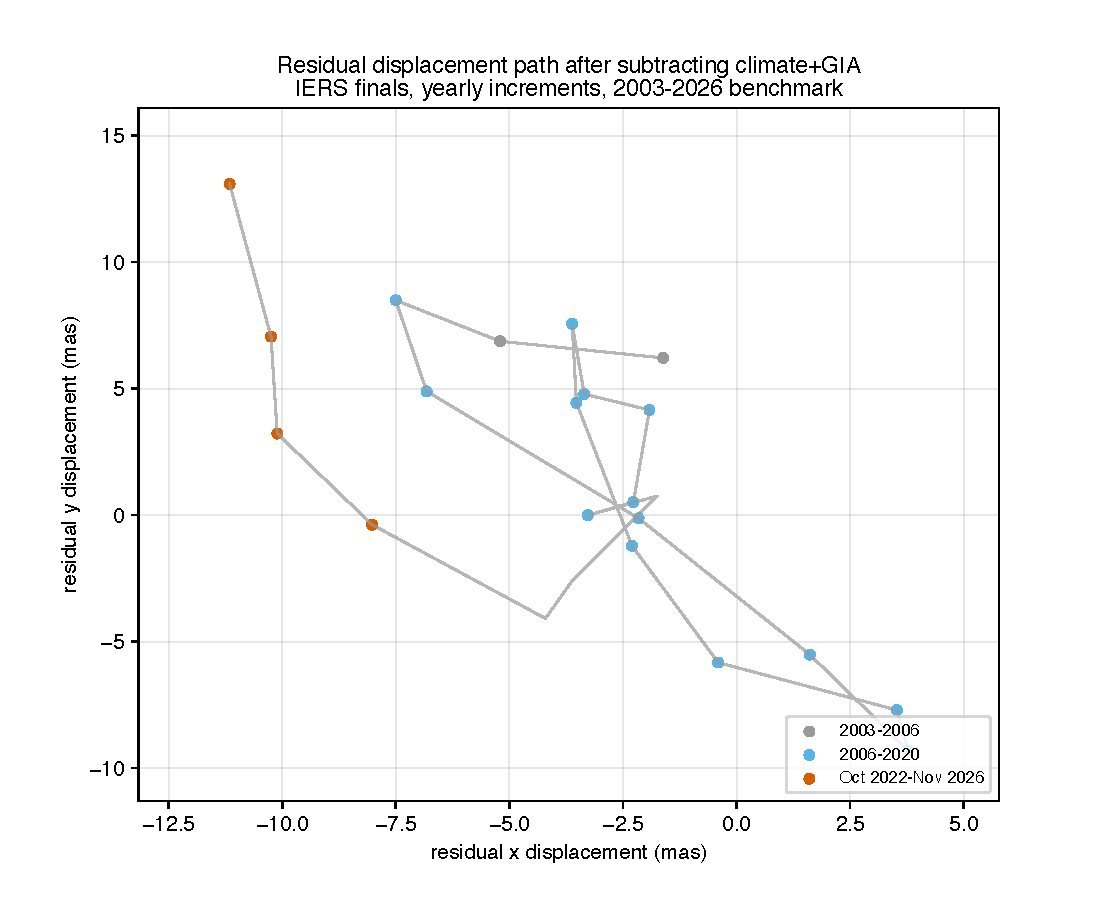
\includegraphics[width=0.9\textwidth]{figures/fig7_residual_path.pdf}
\caption{Residual displacement path in displacement space, IERS finals 2003--2026. Yearly displacement increments are corrected by the known climate+GIA rates (converted to arcsec/yr), and the cumulative residual path is plotted in milliarcseconds; axes are extended so the endpoint is visible rather than hidden under the legend. The path reaches about 17 mas (roughly 0.53 m); the last-year jump is driven by the truncated end. The climate values are measured for 2003--2015 and applied as a benchmark to 2026; the residual includes unmodelled processes and is approximate.}
\label{fig:residual-path}
\end{figure}

The subtraction is a benchmark, not an attribution. The climate reconstruction and GIA trend are measured for 2003--2015 and overlap the baseline period; the residual therefore contains whatever is not captured by those known terms: unmodelled processes. It does not identify a mechanism and does not establish a causal rotational claim. The baseline residual is consistent with zero to about 1 mas/yr over an overlapping benchmark period. Comparison against the IERS Conventions mean-pole model remains the next benchmark and is not performed here.

\section{Reproducibility}

The reproduction script is \texttt{scripts/polar\_drift\_repro.py}. The leap-year denominator is used for the year fraction, which removes duplicate timestamps at year boundaries; the effect on slopes is under about 0.3\%. It loads the dated snapshot by default and reproduces the diagnostics, epoch rates with bootstrap intervals, net displacement, rolling rates, burst sensitivity sweep, baseline residual subtraction and all nine figures; the \texttt{--live} flag fetches the endpoint instead. Run from the paper directory:
{\small
\begin{verbatim}
cd latex/papers/polar_motion_wobble_calibration
FIGGEN=$HOME/.venvs/figgen/bin/python3
$FIGGEN scripts/polar_drift_repro.py
\end{verbatim}
}
The dated snapshot is archived under \texttt{data/} with SHA-256 checksums:

\begin{table}[ht]
\centering
\caption{Dated data snapshot (2026-11-24) and SHA-256 checksums.}
\label{tab:snapshot}
\small
\resizebox{\textwidth}{!}{%
\begin{tabular}{lll}
\toprule
Dataset & Snapshot file & SHA-256 \\
\midrule
IERS finals & \texttt{eop\_finals\_2026-11-24.json} & \texttt{b6baac64fd3472af806f91c1c67a834edee4e1a1ee96357515e0e86f8d2aa8c8} \\
JPL EOP2 & \texttt{eop\_jpl\_2026-11-24.json} & \texttt{05c4546fec4f03dea8661199f8cd21aad81b4b7bc3acbd1f5167431f1edbbace} \\
C04/IAU2000A & \texttt{eop\_c04\_2026-11-24.json} & \texttt{f9e834b008fb696152f29d9d530332ebab5085e446d6ff954b4f51092db84b44} \\
\bottomrule
\end{tabular}}
\end{table}

The full package --- paper source, PDF, figures, snapshot and script --- is published at \url{https://github.com/nobulart/polar-motion.git} \cite{repo}. The script prints assertions for the raw, whole-record co-fit, sequential, smoothed and interior values, verifies each snapshot checksum, and uses 2-year blocks with 3000 bootstrap replicates seeded per call. The \texttt{EXPECTED} hash literals are intact Python strings; the appendix listing's \texttt{breaklines} wraps them visually, not literally. Figure font embedding uses PDF font type 42, verified with \texttt{pdffonts} to carry no Type-3 rows. The paper builds with \texttt{tectonic main.tex} from the paper directory; figures resolve under \texttt{figures/} through the \texttt{graphicspath} declaration.

\section{Calibration limits}

\begin{enumerate}[leftmargin=*]
\item The epoch boundaries are exploratory: a dataset-specific early window, a common 2010--2020 middle window, and a burst window defined after seeing the episode. They are not pre-registered hypotheses.
\item Edge truncation inflates the burst estimate: the full-window smoothed rate is 5.9 mas/yr, the interior-only rate is 3.8 mas/yr, but that interior check spans about 2.1 years and is noisy. The point estimates (3.6, 4.6, 5.9) are monotonic; their intervals overlap and the rolling series does not support a trend.
\item The smoothed series is autocorrelated, so bootstrap intervals are approximate; the bootstrap does not capture the systematic edge bias.
\item The raw 20.0 mas/yr slope is one example of scatter; trailing raw slopes range 1.5--22.8 mas/yr and read 5.0 at the series end.
\item The three products share one observational base (VLBI, GPS, SLR); identical burst values are consistency, not independent corroboration. Before 1973 the JPL and C04 series include optical astrometry with errors of tens of milliarcseconds.
\item The rates are estimates of mean-pole drift. They do not establish coupling, mechanism, or any causal rotational claim; that remains interpretation-tier.
\item The azimuth is signed longitude, east-positive; negative values are west. Reporting magnitudes without the sign loses the direction.
\item The record begins in 1962 (JPL, C04) or 1973 (IERS finals). Totals extending before that span, such as a fifty-foot displacement since 1850, are not testable from this endpoint.
\item No comparison against the IERS Conventions mean-pole model is made here; that is the next benchmark.
\end{enumerate}

\section{Conclusion}

The secular mean-pole drift is small and measurable: roughly 11--16 cm/yr in the early era, 14.3 cm/yr in the common 2010--2020 window, and 18.1 cm/yr in the recent four-year window, with bootstrap intervals spanning 3.6--8.6 mas/yr across products. The point estimates are monotonic, but their intervals overlap and the rolling series does not support a trend. The products share one observational base, so agreement is consistency rather than independent corroboration. Raw and sequential-sinusoid methods inflate the recent rate to 33--62 cm/yr through residual wobble; the centered four-year smoothing reduces it, with the interior-only variant at 11.7 cm/yr (a noisy ~2.1-year check). A whole-record one-basis co-fit with periods in years gives 3.2 mas/yr. The raw 20.0 mas/yr slope is one example of scatter; trailing raw slopes range 1.5--22.8 mas/yr and read 5.0 at the series end. The net displacement since 1962/1973 is 5.94--7.58 m (19.5--24.9 ft), with the recent window adding about 0.74 m in the yearly-mean estimate, which includes the truncated end and is approximate. The snapshot, checksums and script are stated in full so every number can be regenerated.

\begin{thebibliography}{5}
\bibitem{iers} International Earth Rotation and Reference Systems Service. Earth Orientation Parameter products: finals.all IAU1980, finals2000A IAU2000, and EOP 20u24 C04 IAU2000A. Accessed through the DRIFT dashboard endpoint, 24 November 2026.
\bibitem{jpl} Jet Propulsion Laboratory. Earth Orientation Parameters EOP2 (PMx/PMy), daily long and short products. Accessed through the DRIFT dashboard endpoint, 24 November 2026.
\bibitem{drift} Stone, Craig (2026). \emph{DRIFT: A Constraint-First Polar Motion Dashboard}, version 1.6.5. Local dashboard at \url{http://mac-studio:3111}.
\bibitem{adhikari} Adhikari, Surendra and Ivins, Erik R. (2016). Climate-driven polar motion: 2003--2015. \emph{Science Advances} 2(4):e1501693.
\bibitem{repo} Stone, Craig (2026). Wobble-suppressed calibration of mean-pole polar motion: paper, figures, dated snapshot and reproduction script. Public repository at \url{https://github.com/nobulart/polar-motion.git}.
\end{thebibliography}

\appendix
\section{Reproduction code}

The complete reproduction script is included verbatim from \texttt{scripts/polar\_drift\_repro.py}:

\lstinputlisting[language=Python]{scripts/polar_drift_repro.py}

\end{document}
